\section{Merging $k$ Totally Ordered Sets}
\label{tree:merging:kgeq3}

We give the \ITLB and a \BigO{\ITLB} algorithm for Merging. The
algorithm is built on top of the Hwang-Lin algorithm.

\subsection{\ITLB}
\label{tree:merging:kgeq3:ITLB}

Again, we compute the \ITLB as the logarithm of the number of possible solutions
for this problem.
\begin{theorem}[\ITLB for Merging]
The \ITLB for the merging problem when $k \ge 2$ with $|\S_i| = n_i$ and $n =
\sum_{i=1}^{k} n_i$ is \(\log \frac{n!}{n_1! \, n_2! \, \cdots \, n_k!}\).
\end{theorem}
\begin{proof}
We choose the $n_1$ positions among $n$ in $\S'$ for the elements of
$\S_1$ and then recursively make this choice on the remaining $n - n_1$
positions with the elements of \(\S_2 \cup \dots \cup \S_k\). The number of
leaves of the decision tree is $\frac{n!}{n_1! \, n_2! \, \cdots \, n_k!}$. Hence, the
worst-case minimal height of the tree is $\log \frac{n!}{n_1! \, n_2! \, \cdots
\, n_k!}$.
\end{proof}

Note that giving $\log \frac{n!}{n_1! \, n_2! \, \cdots \, n_k!}$ in the form of the
Stirling's approximation gives us \(n \log n - \sum_{i=1}^{k} n_i \log n_i -
\BigO{n}\)
which clearly expresses the information contained in the sorted list $\S'$ of
$n$ elements minus the information we already have.

\subsection{An Algorithm for the Merging Problem}
\label{tree:merging:kgeq3:alg}

We start with the pseudo-code description of our algorithm. We then prove this
algorithm solves the merging problem using \BigO{\ITLB} queries.
\begin{algorithm}[Algorithm for the merging problem]
\item[1.] Let \(\S_i\) and \(\S_j\) be two smallest sets from \(\S_1 ,
\dots , \S_k\).
\item[2.] Merge \(\S_i\) and \(\S_j\) with a \BigO{\ITLB} algorithm.
\item[3.] Merge \((\enum{\S_1 , \dots , \S_k} \setminus \enum{\S_i,\S_j} )
\cup \enum{\S_i \cup \S_j}\).
\end{algorithm}

We use tools from Information Theory to prove that this algorithm has
a query complexity of \BigO{\ITLB}. The first tool we use is Shannon's entropy of a random
variable \(X\), \(H(X)\)
\begin{definition}[Shannon's entropy]
\begin{displaymath}
H(X) \bydef \sum_{x_i} p(x_i) \log \frac{1}{p(x_i)}.
\end{displaymath}
\end{definition}
The second is Huffman codes.

Let us take some time to expose the relation between constructions of Huffman
codes and runs of our algorithm. First, we define the problem of optimal
coding of a random variable with respect to the average length of the messages
encoding events emitted by this random variable. We assume the channel we
use to transmit our messages is perfect.
\begin{problem}[Optimal coding of a random variable]
Given a random variable \(X\) with possible events \(x_1,\ldots,x_n\) occurring
with probability \(0 < p(x_i) \le 1, \sum_{x_i} p(x_i) = 1\), construct an
instantaneous code, \ie a code where no code word is a prefix of another code
word, to transmit events through a perfect channel with alphabet
\(\Sigma = \enum{0,1}\) that minimizes the average size of a message encoding
an event.
\end{problem}

The are several results on this subject which we summarize in the
following theorem.
\begin{theorem}[Optimality of Huffman codes]
If we define \(l(x_i)\) to be the code
length for event \(x_i\), then the average code length is
\begin{displaymath}
L(X) = \sum_{x_i} p(x_i) l(x_i).
\end{displaymath}
The average code length \(L(X)\) of any instantaneous coding scheme cannot be
less than
the entropy of the random variable \(H(X)\).
With respect to the objective function we mentioned above, Huffman coding is
an optimal instantaneous code and its average length \(L_H(X)\) is bounded by
\begin{displaymath}
H(X) \le L_H(X) \le H(X) + 1.
\end{displaymath}
\end{theorem}

\(L_H(X)\) is achieved by constructing a Huffman tree. The method to build this
tree is the following. We start with \(n\) leaves, one for each possible event
\(x_i\). We assign a weight of \(p(x_i)\) to each of these leaves. The current
structure is not quite a tree but a pool of disconnected nodes. We
replace two nodes of the pool with smallest weight by a new one which
acts as their parent in the Huffman tree. The weight of this new node is
the sum of the weights of its children. We repeat this
replacement operation until the pool contains only one element. This last
element is the root of the tree. Since at each step we replace two nodes by
one, after \(n-1\) of these steps the tree is constructed.

We make the parallel with our merging algorithm. If we want to merge
multiple totally ordered sets \(\S_1,\ldots,\S_k\) having different lengths we can use a similar
approach. To each set \(\S_i\) we assign a fake event with probability
\(\frac{\card{\S_i}}{n}\). The Shannon entropy of the random variable
\(S\) having this probability distribution is
\begin{align*}
H(S) &= - \sum_i \frac{\card{\S_i}}{n} \log \frac{\card{\S_i}}{n}\\
&= - \sum_i \frac{\card{\S_i}}{n} (\log \card{\S_i} - \log n)\\
&= \sum_i \frac{\card{\S_i}}{n} \log n - \sum_i \frac{\card{\S_i}}{n} \log \card{\S_i}\\
&= \frac{1}{n} \sum_i \card{\S_i} \log n - \frac{1}{n} \sum_i \card{\S_i} \log
\card{\S_i}\\
&= \frac{1}{n} (n \log n - \sum_i \card{\S_i} \log \card{\S_i}).
\end{align*}

The definition of \(p(\S_i)\) is consistent with the invariant of
the Huffman tree construction algorithm since merging two totally ordered sets
\(\S_i\) and \(\S_j\) produces a new one of size \(\card{\S_i} + \card{\S_j}\).

We prove that for a merging algorithm that would iteratively merge the two
smallest remaining totally ordered sets, the number of comparisons used is at
most \(n L_H(\S)\). To make this explicit, we rearrange the terms of \(L_H(\S)\),
\begin{displaymath}
L_H(\S) = \sum_i \frac{\card{\S_i}}{n} l(\S_i) = \frac{1}{n} \sum_i l(\S_i) \card{\S_i}.
\end{displaymath}

In the equation above, \(l(\S_i)\) corresponds to the number of times elements
of \(\S_i\) are taking part in a merge operation. When merging two totally
ordered sets \(\S_i\) and \(\S_j\) the standard \tapemerge algorithm uses less
than \(\card{\S_i} + \card{\S_j}\) comparisons. Moreover, the totally ordered set
associated to a node of the Huffman tree is the union of the totally ordered
sets associated to \(u\) leaves of the tree. These leaves are
\(\S_{i_1},\ldots,\S_{i_u}\) and have lengths
\(\card{\S_{i_1}},\ldots,\card{\S_{i_u}}\). When two nodes are merged, it
requires thus less than
\(\card{\S_{i_1}}+\cdots+\card{\S_{i_u}}+\card{\S_{j_1}}+\cdots+\card{\S_{j_v}}\)
comparisons. We can rearrange these \(\card{\S_{i_w}}\) and conclude that
\(\sum_i l(\S_i) \card{\S_i}\) is an upper bound on the number of comparisons used
by our algorithm. Since
\begin{displaymath}
n H(\S) \le n L_H(\S) \le n H(\S) + n,
\end{displaymath}
our algorithm requires at most \(n \log n - \sum_i \card{\S_i} \log \card{\S_i} +
n\) comparisons which is \(\ITLB + \BigO{n}\).

To handle sublinear \ITLB we need to resort to a last trick. The only
way the \ITLB can be \SmallO{n} is if the last two nodes \(\U\) and
\(\L\) we merge have sizes \(m\) and \(n\) respectively such that \(m =
\SmallO{n}\). Otherwise merging them would require \BigOmega{n} comparisons.
If \(m = \SmallO{n}\), then we can use the Hwang-Lin algorithm to merge those
two nodes using \(\BigO{m \log \frac{n}{m}} = \BigO{\ITLB}\) comparisons. Moreover, the set
\(\L\) can only be a leaf of the Huffman tree. Indeed, it cannot be the result
of a merge operation between two \BigO{m} sized nodes. Since this is the only
kind of merge operation that is allowed before having merged the set \(\U\)
with another one, \(\L\) is necessarily a leaf. Since producing the totally ordered
set of size \(m\) uses at most \BigO{\ITLB} comparisons using our
previous algorithm, after trading
\tapemerge for the Hwang-Lin algorithm we get an algorithm
solving the merging problem using \BigO{\ITLB} queries.

Our algorithm is thus building the Huffman tree and then merges the two deepest
leaves of the Huffman tree using the Hwang-Lin algorithm until there is only
one leaf left.

\begin{figure}
	\centering
	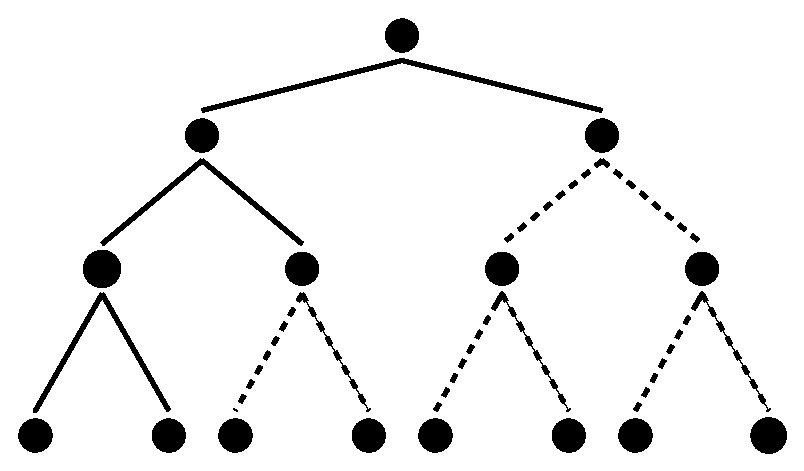
\includegraphics[width=0.4\textwidth]{fig/merging/huffman-2-trim}
	\caption{Complexity of the merging problem as a difference between the whole merge process and its subprocesses.}
	\label{tree:merging:fig/huffman-2}
\end{figure}

We provide a visual way of understanding these results. Looking at
\ref{tree:merging:fig/huffman-2} we can deduce the complexity of the algorithm.
The dashed lines in \ref{tree:merging:fig/huffman-2} represent steps producing
information we already have. Since those steps do not need to be processed, and
since they normally would have required us to use \(\BigO{n \log n}\) queries, we have a
total complexity of $\log n! - \sum_{i=1}^{k} \log n_i! = \ITLB$, where $n_i$ is the cardinality of the $i$-th totally ordered set
of the input.
